\section{Fractal tesseract topology with jitter}\label{sec:fractal-tesseract-jittering}

\paragraph{Fractal tesseract.}
The fractal tesseract is the self-similar branch/hinge/branch topology of recursive cut-running. Recursive cut-running preserves branch, hinge, and branch across nested presentations. Each retained occurrence inherits \(x\succ x=x\) and can run the cut again. The result is recursive incidence, return, and enclosure.

\paragraph{Jitter.}
Jitter is unresolved successor movement inside the fractal tesseract topology. Before a carried current has seated, the next branch/hinge/branch continuation can remain unsettled. Jitter is the local motion of successor possibility before return stabilizes.

\paragraph{Finite \(\Qfour\) witness.}
A finite \(\Qfour\) chart is a local witness of the fractal tesseract topology. A resolved duon has four active dion positions and one carried monon hinge. Partial unspooling of the four active positions gives \(\{0,1\}^4\). Hamming-1 adjacency gives \(\Qfour\). The middle hinge remains the ternary fibre.


\paragraph{Four-edge \(x\) witness.}
A retained \(x\)-occurrence in the finite \(\Qfour\) witness is a vertex
\[
\epsilon=(\epsilon_1,\epsilon_2,\epsilon_3,\epsilon_4)\in\{0,1\}^4.
\]
The four active dion positions supply the four tesseract-edge directions:
\[
\epsilon \leftrightarrow \epsilon\oplus e_i,
\qquad i=1,2,3,4.
\]
Thus every retained \(x\)-vertex in the local witness has
\[
\deg_{\Qfour}(\epsilon)=4.
\]
The monon hinge \(\mu\) remains the ternary fibre over that four-edge support. This is the finite witness for the sketch statement that a retained \(x\) carries four tesseract edges.

\begin{figure}[H]
\centering
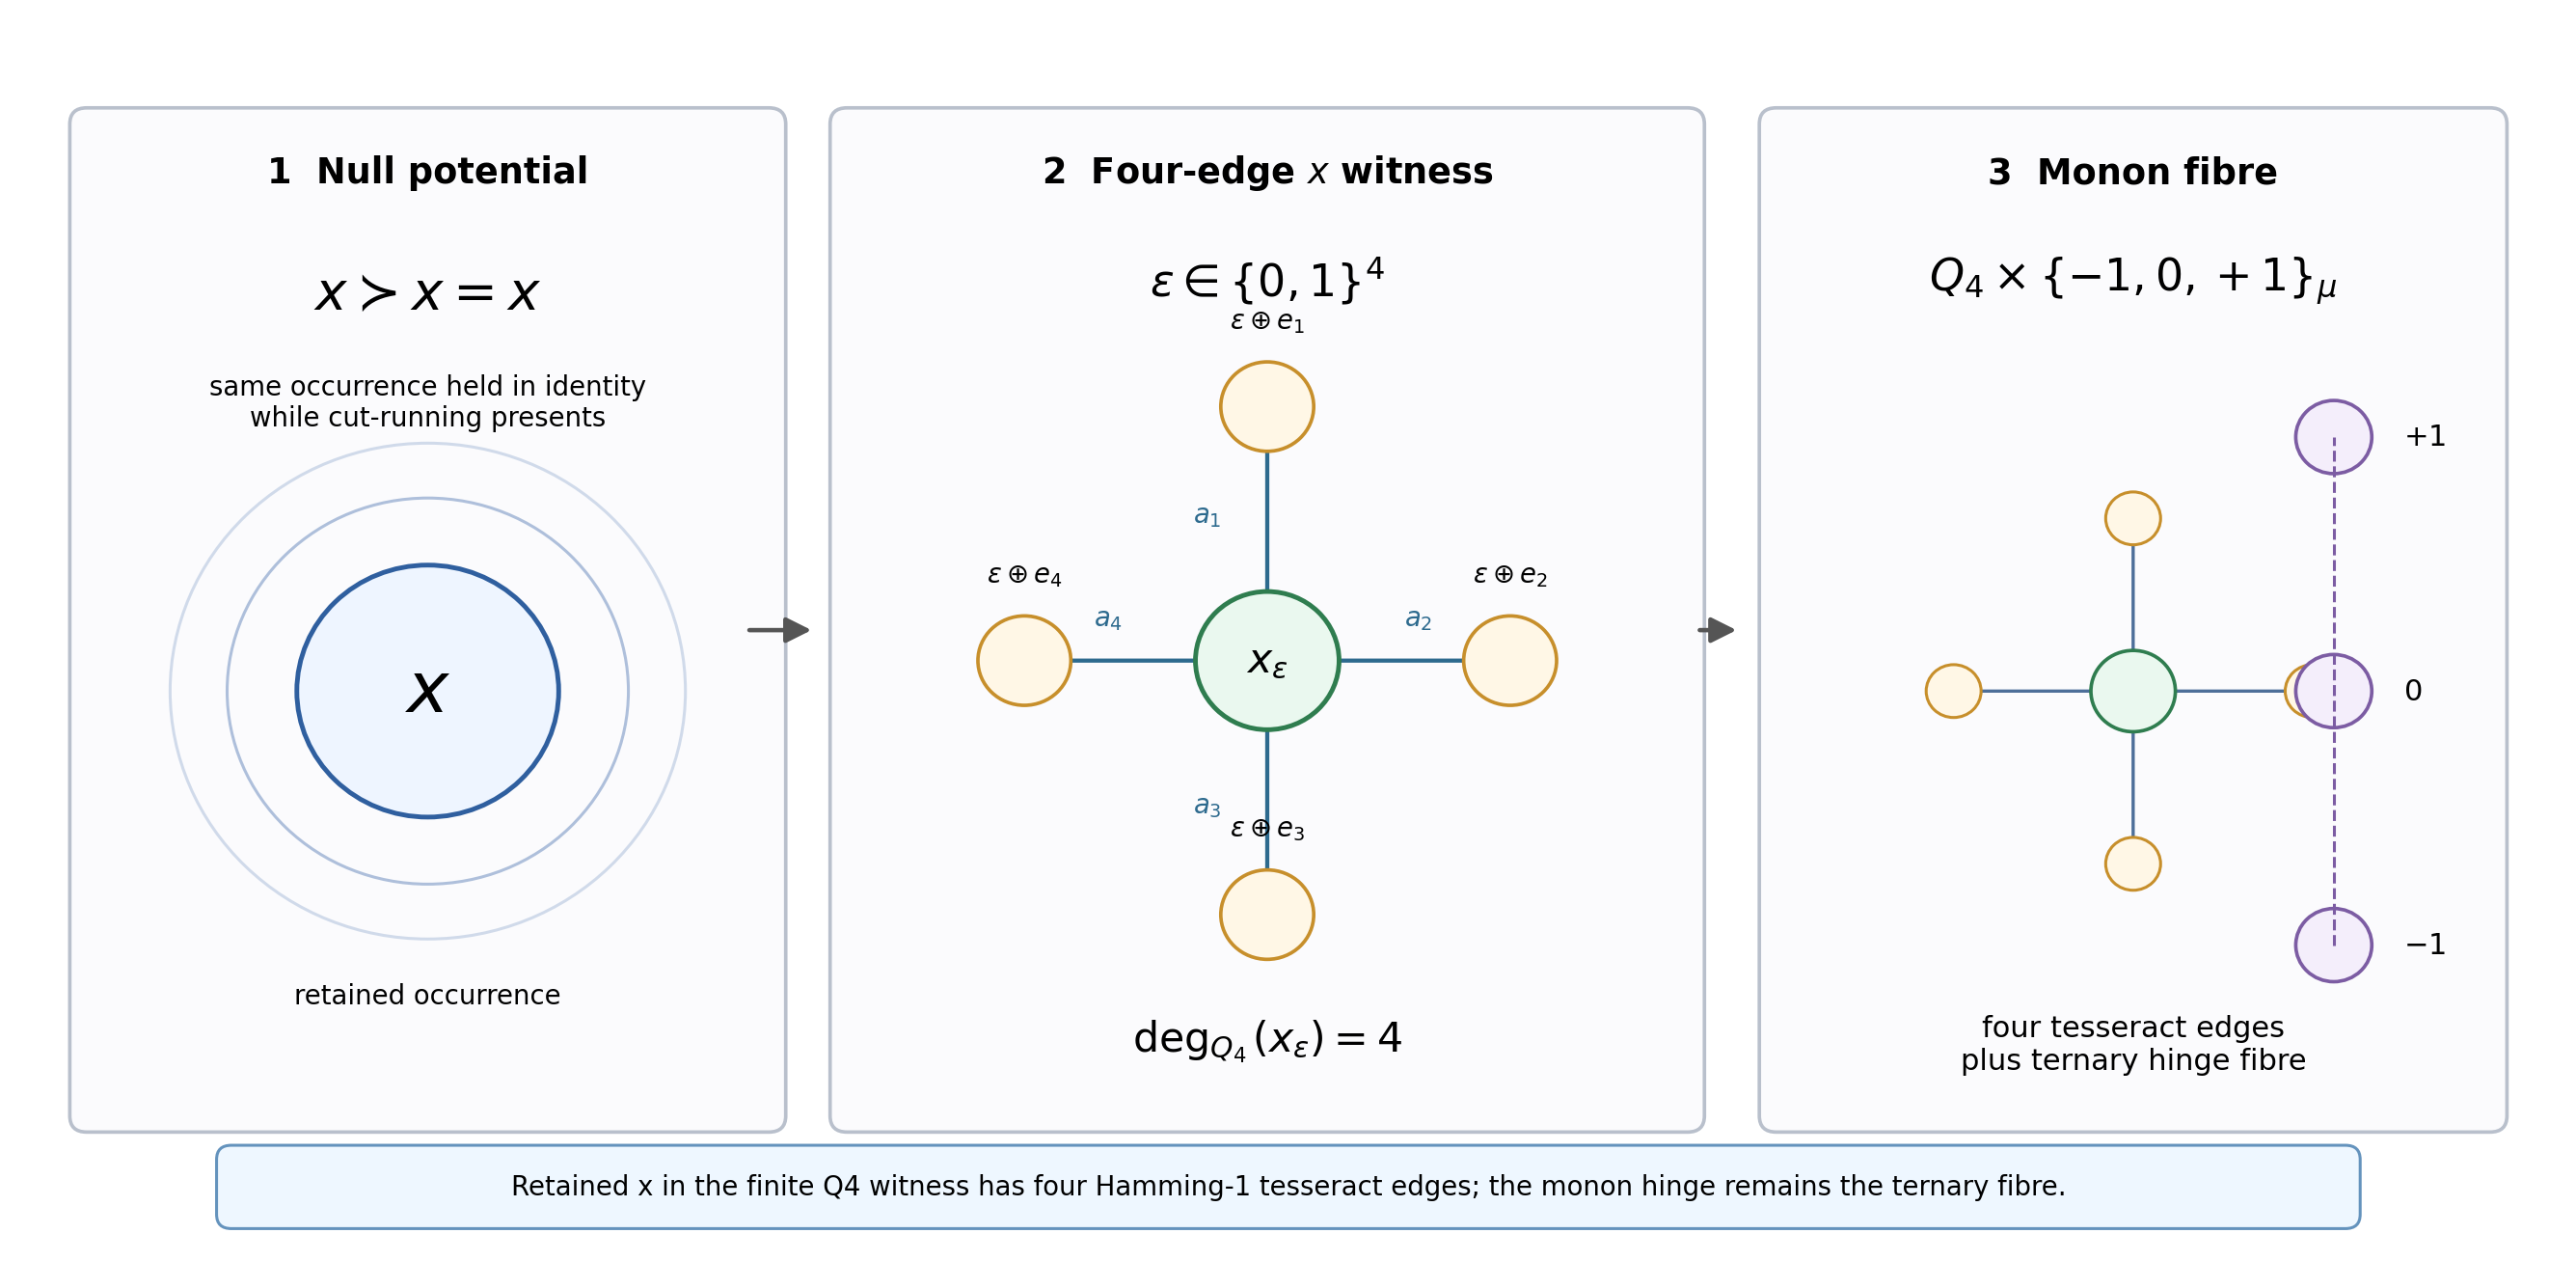
\includegraphics[width=0.96\linewidth]{figures_jpg/v39_18_null_four_edge_x_witness.png}
\caption{Null-to-tesseract four-edge witness. The retained \(x\) becomes a vertex of the finite \(\Qfour\) chart; its four Hamming-1 edges are the active tesseract directions, and the monon hinge remains the ternary fibre.}
\label{fig:null-four-edge-x-witness}
\end{figure}

\paragraph{Fractal address.}
The fractal address is four-nary even:
\[
\mathbf a\in\mathcal A^{\mathrm{even}}_4.
\]
The origin anchor is \(\mathtt{00}\). Retained closure addresses begin
\[
\mathtt{00},\ \mathtt{02},\ \mathtt{10},\ \mathtt{12},\ \mathtt{20},\ \mathtt{22},\ \mathtt{30},\ \mathtt{32},\ \mathtt{100},\ldots .
\]
The address records retained closure positions of the fractal tesseract topology.

\begin{figure}[H]
\centering
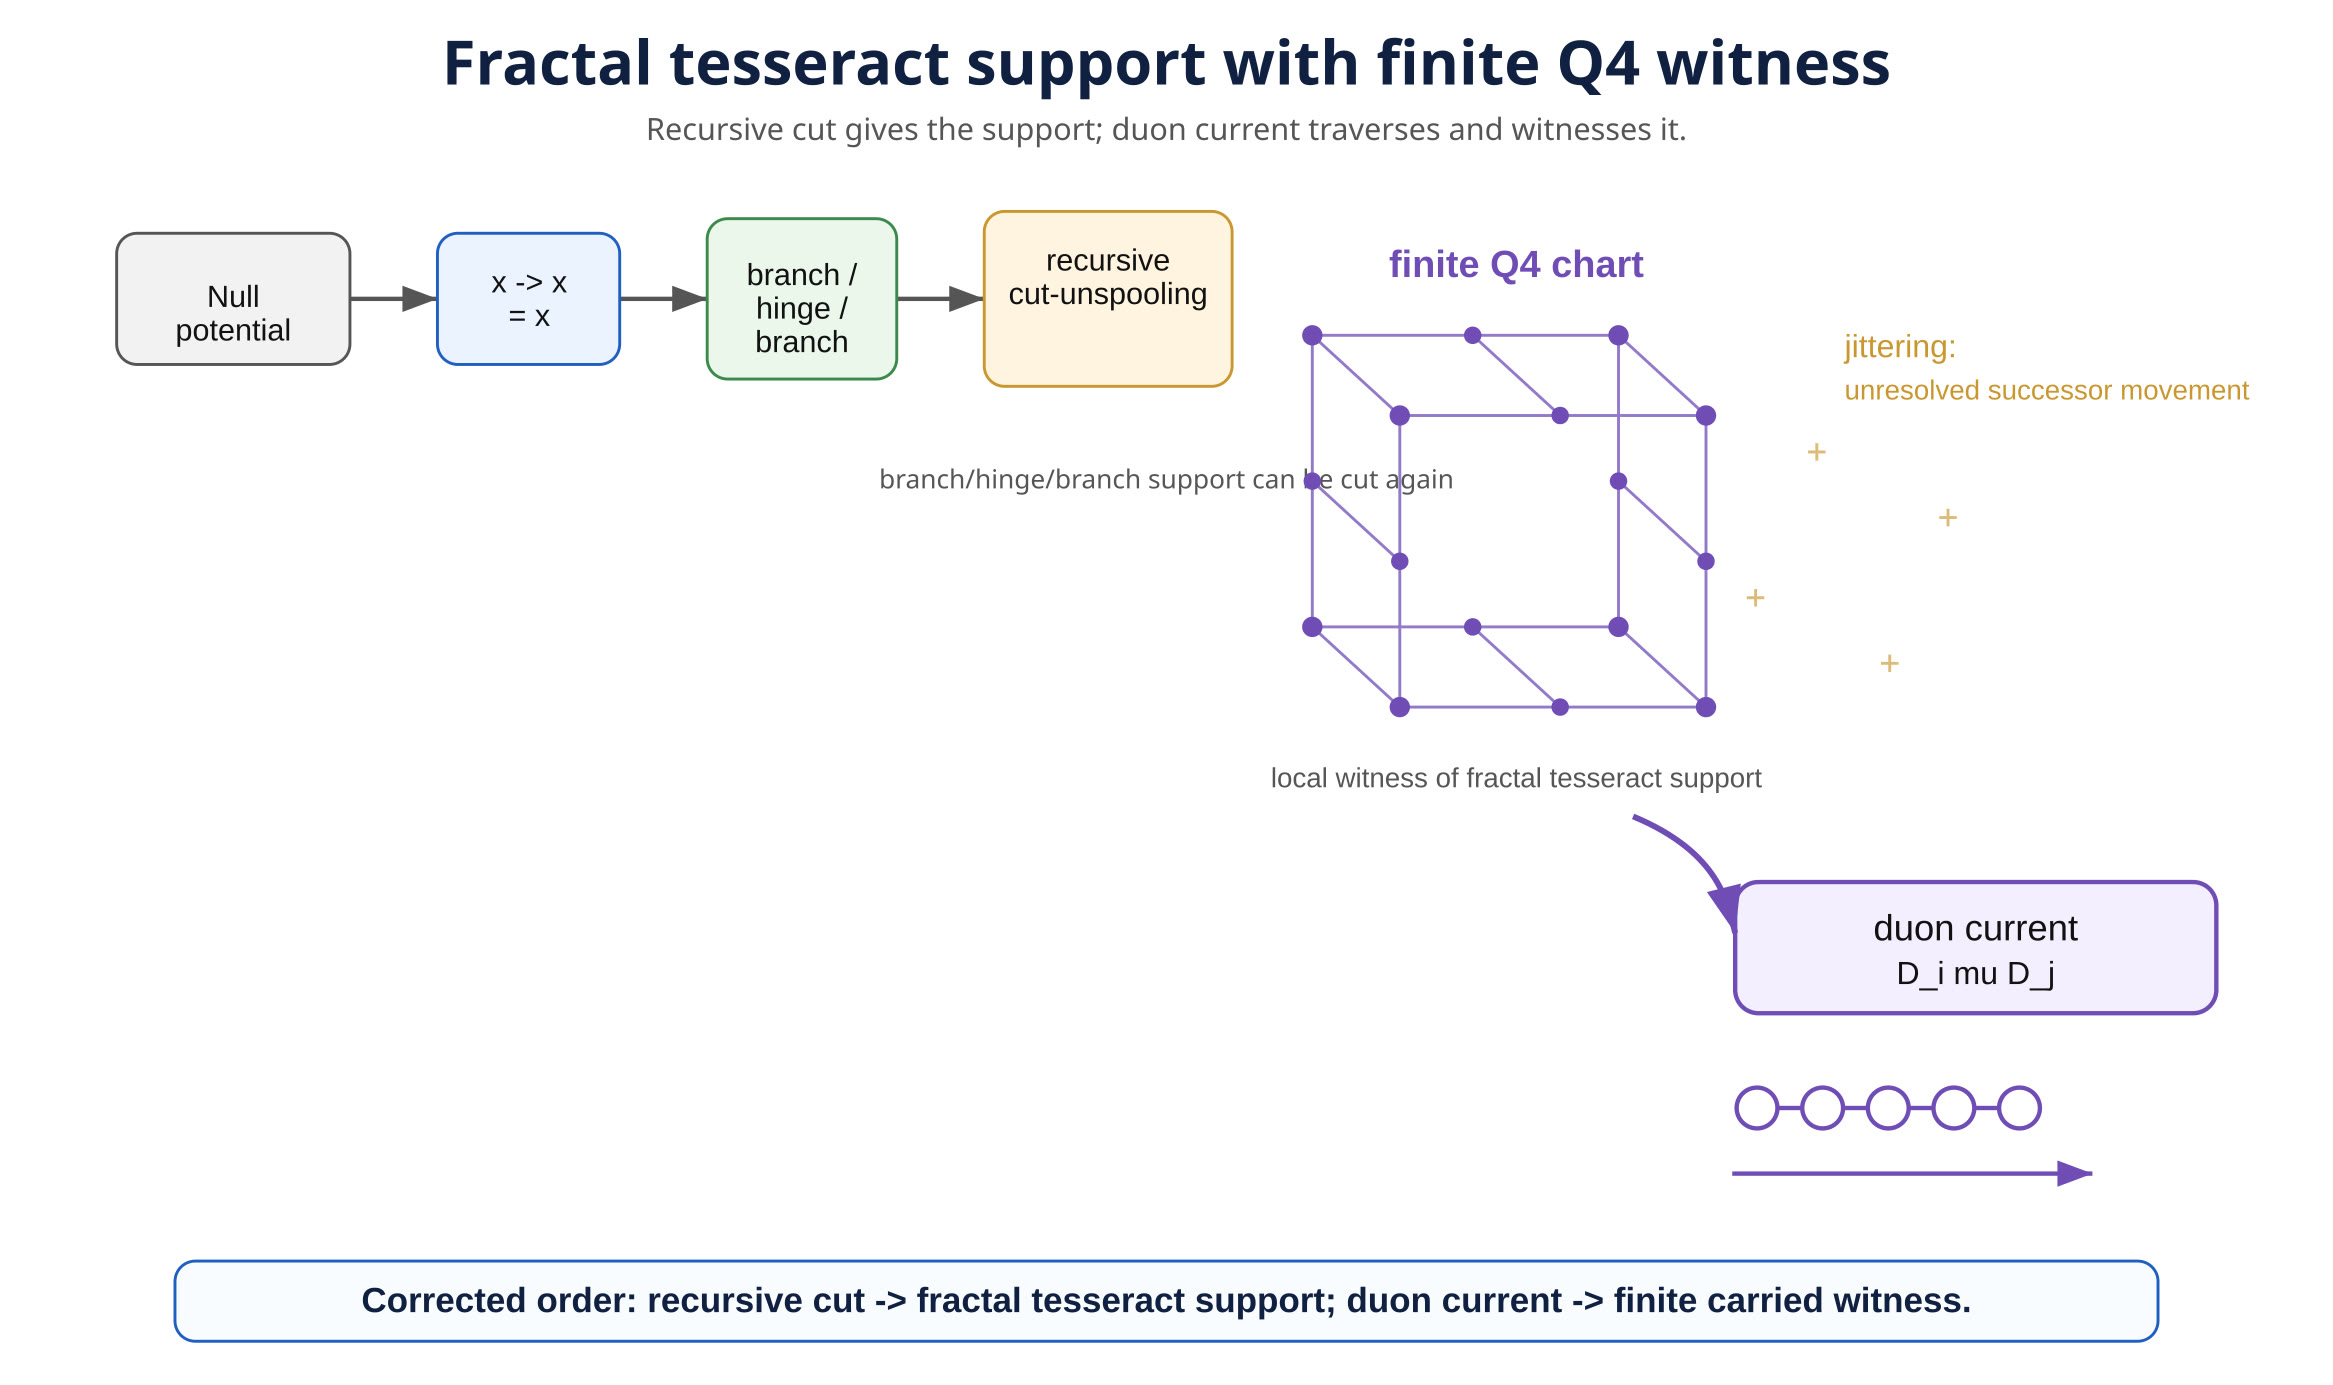
\includegraphics[width=0.96\linewidth]{figures_jpg/v39_fractal_tesseract_q4_witness.jpg}
\caption{Fractal tesseract support with finite \(\Qfour\) witness. Recursive cut-running supplies the topology; duon current later traverses and witnesses that topology as carried hinge-current.}
\label{fig:v39-fractal-tesseract-q4-witness}
\end{figure}
